\section{Reconfiguration-induced Deadlock}\label{sec:reconfigdeadlock}



While PFC deadlock can be avoided by leveraging a routing function that introduces no cycle in the buffer dependency graph. However, this approach cannot eliminate the cyclic buffer dependency that may arise during routing reconfiguration process.

In this part, we use examples to show 1) cyclic buffer dependency can be generated for both tree based and non-tree based DCNs when the routing reconfiguration is not well planed; 2) a bad deadlock-free reconfiguration plan will lead to a slow reconfiguration process.

\subsection{Deadlock Under Tree Based DCNs}\label{subsec:treecase}

\begin{figure}[t]
	\centering
	
	\subfloat[short for lof][Initial routing configuration.] {
		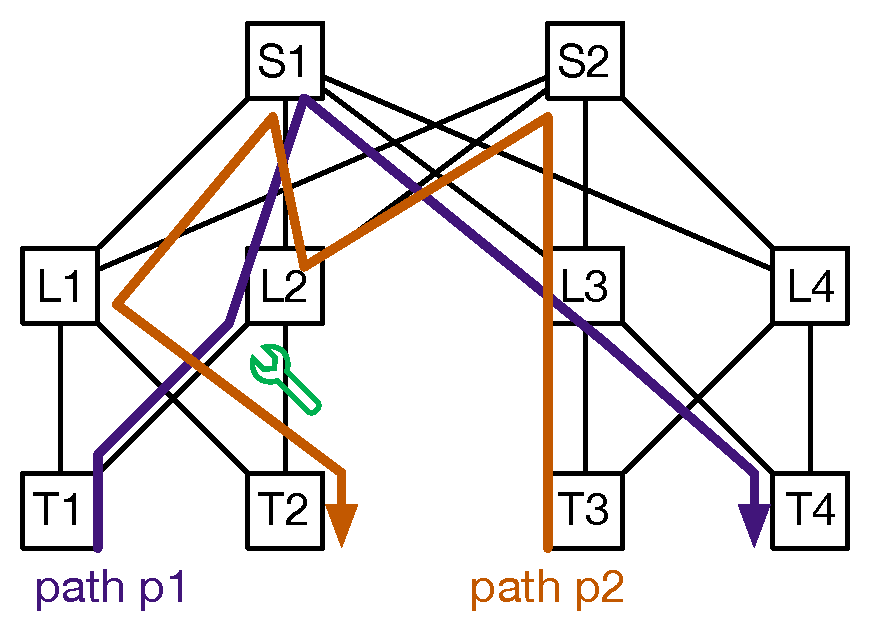
\includegraphics[width=0.24\textwidth] {figs/deadlock_tree_a}
	}
	\subfloat[short for lof][Routing configuration after reconfiguration.]{
		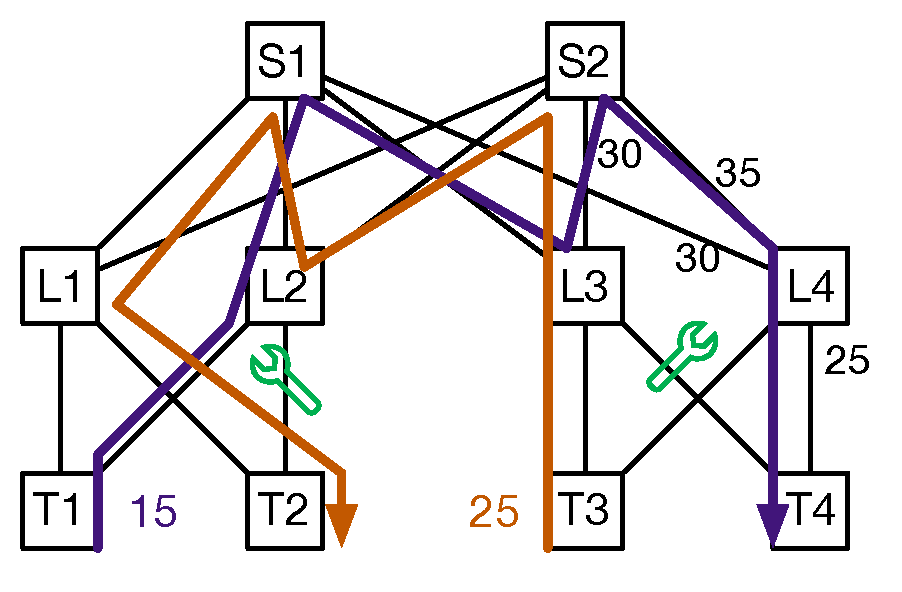
\includegraphics[width=0.24\textwidth] {figs/deadlock_tree_b}
	}
	
	\vspace{-0.1in}
	\subfloat[short for lof][Intermediate routing configuration 1.] {
		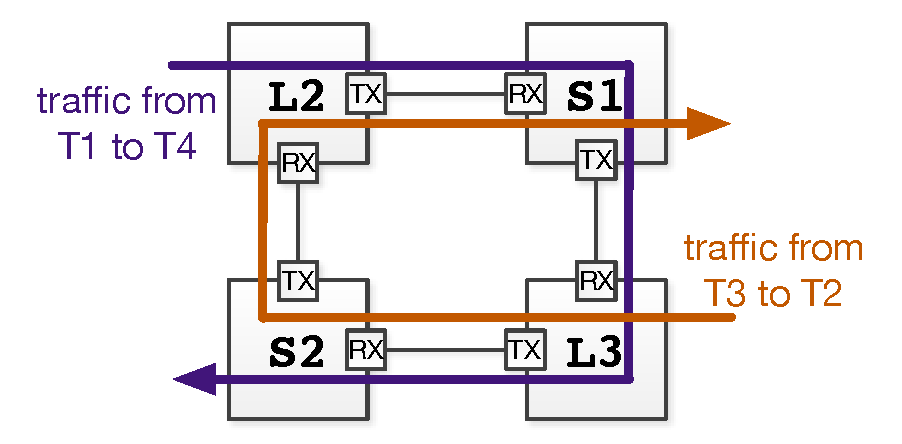
\includegraphics[width=0.24\textwidth] {figs/deadlock_tree_c}
	}
	\subfloat[short for lof][Intermediate routing configuration 2.] {
		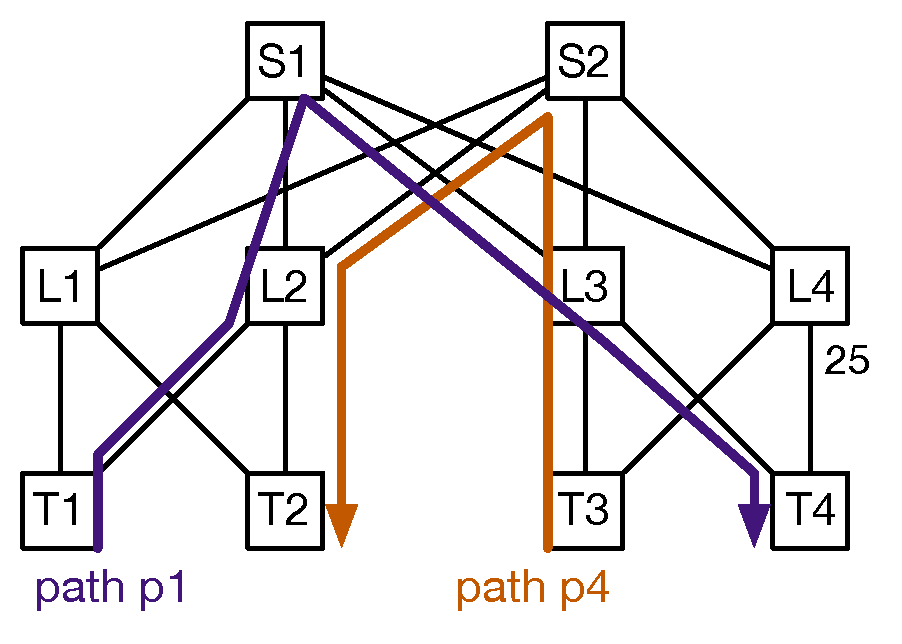
\includegraphics[width=0.24\textwidth] {figs/deadlock_tree_d}
	}
	
	
	\vspace{-0.1in}
	\subfloat[short for lof][Buffer dependency graph.]{
		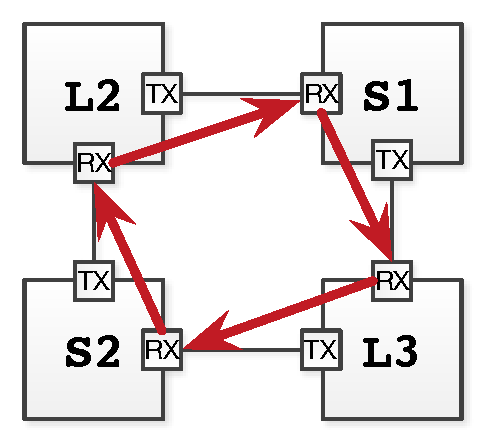
\includegraphics[width=0.2\textwidth] {figs/deadlock_tree_e}
	}
	\subfloat[short for lof][Deadlock-free reconfiguration schemes.] {
		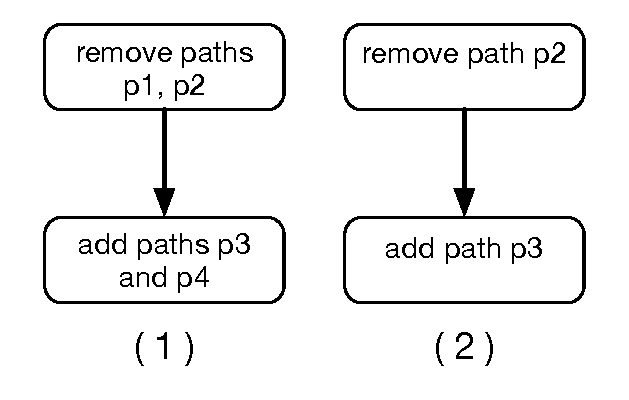
\includegraphics[width=0.28\textwidth] {figs/treecase_dfschemes}
	}
	
	\caption{Reconfiguration-induced deadlock case for tree topology.}\label{fig:treecase}
	\vspace{-0.2in}
\end{figure}

Fig.~\ref{fig:treecase}(a) shows a small Leaf-Spine topology, which is a typical tree based DCN topology.

\textbf{Reconfiguration scenario:} For maintenance reason, the network operator now wants to replace two links L2-T2 and L3-T4 in the network. The link replacement is scheduled to be executed with two steps. The first step is to replace link L2-T2, and the second step is to replace link L3-T4.

To avoid long-term packet loss during link replacement, the network traffic passing through the operated link needs to be migrated to some other paths. 

In the first step, part of the traffic from switch T3 to switch T2 is migrated to a non-shortest path p2 because link L2-T2 is down and the alternative shortest paths cannot accommodate all the traffic, as shown in Fig.~\ref{fig:treecase}(a). In the second step, part of the traffic from switch T1 to switch T4 is migrated to a non-shortest path p3 because link L3-T4 is down and the alternative shortest paths cannot accommodate all the traffic, as shown in Fig.~\ref{fig:treecase}(b).

Let $R_{old} = \{p1, p2\}$, and $R_{new} = \{p3, p4\}$. It is easy to check both $R_{old}$ and $R_{new}$ are deadlock-free routing functions. 

\textbf{Cyclic buffer dependency during reconfiguration process:} In order to proceed from the first step to the second step, a routing reconfiguration is required to transition the routing function from $R_{old}$ to $R_{new}$.

During the reconfiguration process, different executed orders of configuration operations will lead to different intermediate routing functions. Specifically, if path p3 is added to the routing function before path p2 is removed, the intermediate routing configuration shown in Fig.~\ref{fig:nontreecase}(c) will be created. If path p4 is added to the routing function before path p1 is removed, the intermediate routing configuration shown in Fig.~\ref{fig:nontreecase}(d) will be created.  

The intermediate routing configuration shown in Fig.~\ref{fig:nontreecase}(c) introduces a cyclic buffer dependency.  To help readers understand this, in Fig.~\ref{fig:treecase}(e), we draw the buffer dependency among four switches L2, L3, S1 and S2. We reposit the locations of these four switches and draw both ingress queues (RX) and egress queues (TX) for the purpose of better explanation. As we can see, there is a cyclic buffer dependency among the ingress queues. This indicates that the network is now exposed to the danger of PFC deadlock.

\textbf{Deadlock-free reconfiguration schemes:} In Fig.~\ref{fig:nontreecase}(f), we present two possible deadlock-free reconfiguration schmes. The first scheme is to remove all the paths in $R_{old}$ before adding any new paths in $R_{new}$. This scheme will lead to a slow reconfiguration process as all the operations of adding new paths are delayed by the operations of removing old paths. 

The second scheme only requires path p2 to be removed before path p3 is added. All the other paths not mentioned can be updated freely without any order constraint. Hence the speed of routing reconfiguration can be improved.


\subsection{Deadlock Under Non-tree Based DCNs}\label{subsec:nontreecase}

\begin{figure}[t]
	\centering
	
	\subfloat[short for lof][4-node network \textbf{N}.] {
		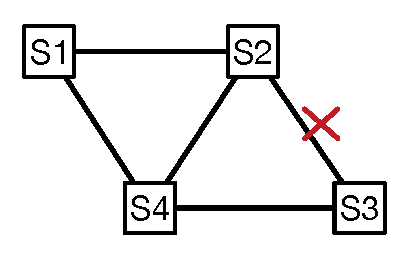
\includegraphics[width=0.16\textwidth] {figs/deadlock_nontree_a}
	}
	\subfloat[short for lof][Spanning tree \textbf{T1}.]{
		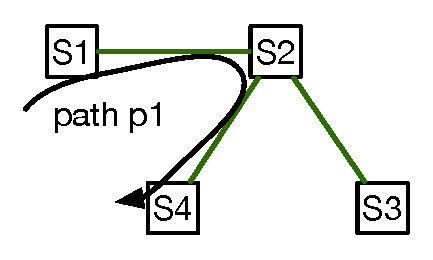
\includegraphics[width=0.16\textwidth] {figs/deadlock_nontree_b}
	}
	\subfloat[short for lof][Spanning tree \textbf{T2}.]{
		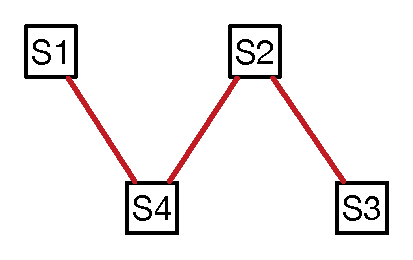
\includegraphics[width=0.16\textwidth] {figs/deadlock_nontree_c}
	}
	
	\vspace{-0.1in}
	\subfloat[short for lof][Spanning tree \textbf{T3}.] {
		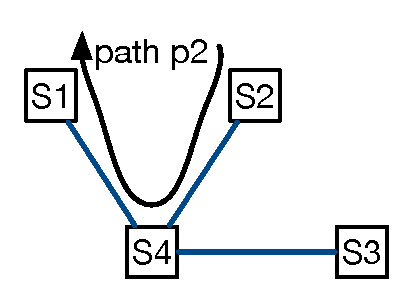
\includegraphics[width=0.16\textwidth] {figs/deadlock_nontree_d}
	}
	\subfloat[short for lof][Spanning tree \textbf{T4}.] {
		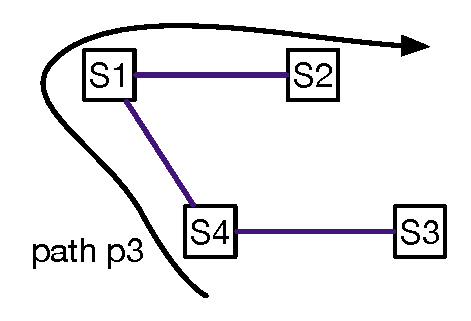
\includegraphics[width=0.16\textwidth] {figs/deadlock_nontree_e}
	}
	\subfloat[short for lof][Buffer dependency graph.]{
		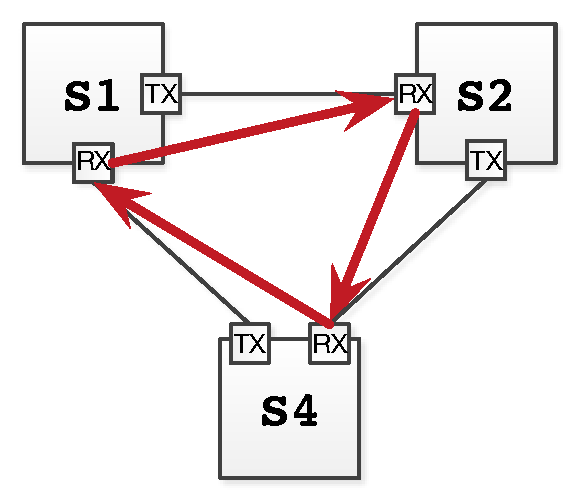
\includegraphics[width=0.15\textwidth] {figs/deadlock_nontree_f}
	}
	
	\caption{Reconfiguration-induced deadlock case for non-tree topology.}\label{fig:nontreecase}
	\vspace{-0.2in}
\end{figure}

As shown in Fig.~\ref{fig:nontreecase}(a), in this example we consider a 4-node network N. This topology can be a subgraph of many non-tree based DCNs, like HyperX~\cite{hyperx}, Jellyfish~\cite{jellyfish} and BCube~\cite{bcube}.

Fig.~\ref{fig:nontreecase}(b)-(e) are four spanning trees \textbf{T1}-\textbf{T4} which specify the routing paths that can be used in N. For example, path p1 is a legal routing path specified in \textbf{T1}.  We use $R_i$ to denote the set of paths specified in tree \textbf{Ti}. Let $R_{old} = R_1 \cup R_2$, and $R_{new} = R_3 \cup R_4$. It is easy to check both $R_{old}$ and $R_{new}$ are deadlock-free routing functions. 

\textbf{Reconfiguration scenario:} Initially, $R_s$ are used as the routing function of N. Due to the failure of link S2-S3, switch S3 becomes unreachable. To maintain connectivity of the network, network operator now wants to perform a routing reconfiguration to transition the routing function from $R_{old}$ to $R_{new}$.

\textbf{Cyclic buffer dependency during reconfiguration process:} During the reconfiguration process, if path p2 in \textbf{T3} and path p3 in \textbf{T4} are added to the routing function before path p1 in \textbf{T1} is removed, a cyclic buffer dependency will be generated, as shown in Fig.~\ref{fig:nontreecase}(f).

\textbf{Deadlock-free reconfiguration schemes:} In Fig.~\ref{fig:dfschemes}, we present three possible deadlock-free reconfiguration schmes. The first scheme is to remove all the paths in \textbf{T1} and \textbf{T2} before adding any new paths in \textbf{T3} and \textbf{T4}. This scheme will lead to a slow reconfiguration process as all the operations of adding new paths are delayed by the operations of removing old paths. 

The second scheme only requires path p1 to be removed before paths p2 and p3 are added. All the other paths not mentioned can be updated freely without any order constraint. Hence the speed of routing reconfiguration can be improved. The third scheme is an optimized reconfiguration scheme in terms of imposing minimum order constraints on the configuration operations. The intuition here is that as long as paths p1, p2 and p3 do not take effect at the same, deadlock-free can be well guaranteed. 



\begin{figure}[t]
	\centering
	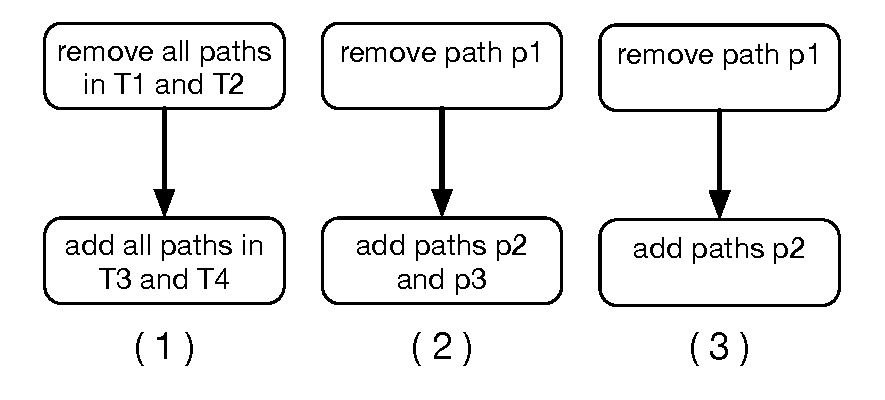
\includegraphics[width=0.45\textwidth] {figs/nontreecase_dfschemes}
	\caption{Three deadlock-free reconfiguration schemes.}\label{fig:dfschemes}
	\vspace{-0.2in}
\end{figure}

%While for this example it may seem easy to find a deadlock-free reconfiguration scheme that requires minimum order constraints, in general it is difficult as there are combinatorial such schemes to be checked.




%\subsection{Measurement of Rule Update Time}\label{subsec:updatetime}
%
%In this part, we demonstrate that adding order constraints to the update of switch rules will significantly prolong the reconfiguration process.
%
%In Fig.~\ref{fig:deadlock_case}, we use a simple example to show how  deadlock can be created when there is a cyclic buffer dependency among a set of switch buffers.
%
%\begin{figure}[t]
%	\centering
%	
%	\subfloat[short for lof][Topology and flows.] {
%		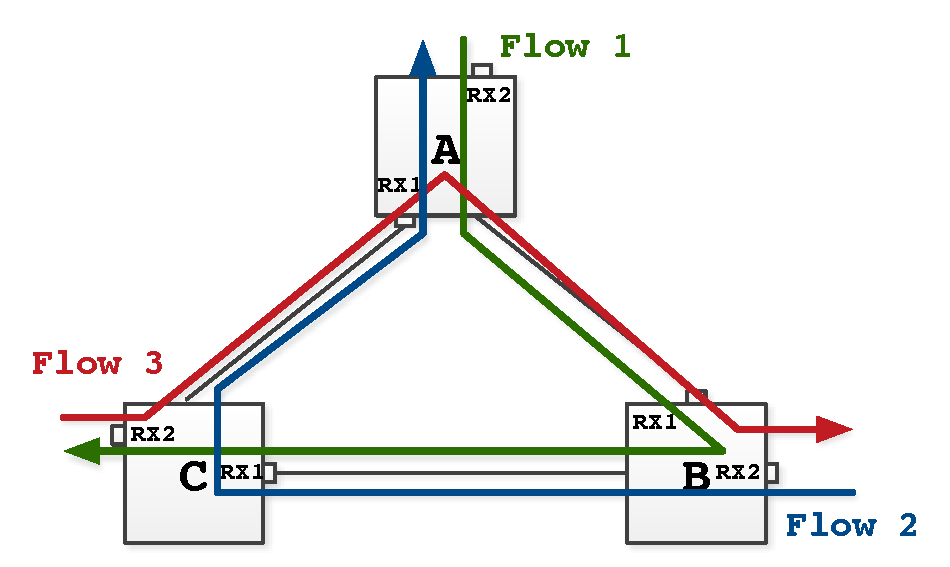
\includegraphics[width=0.3\textwidth] {figs/case1_topo}
%	}
%	\subfloat[short for lof][Buffer dependency graph.]{
%		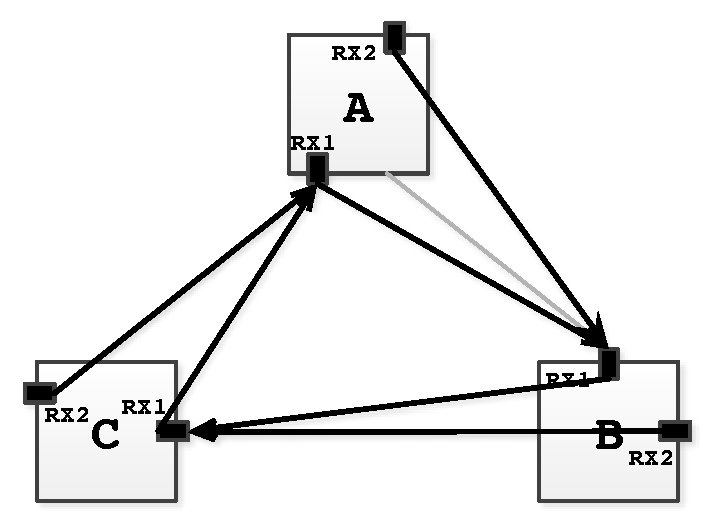
\includegraphics[width=0.2\textwidth] {figs/case1_dependency}
%	}
%	
%	\caption{Flows 1, 2 and 3 forms a cycle in the buffer dependency graph that can create a routing deadlock. In both figures, RX represents an ingress switch queue.}\label{fig:deadlock_case}

%\end{figure}
%
%As shown in Fig.~\ref{fig:deadlock_case}(a), three flows are runing over three switches A, B and C. Flow 1 starts at a host (not shown) attached to A, passes through B, and ends at a host attached to C. Flow 2 and flow 3 are two symmetric flows of flow 1. Buffer dependencies among active ingress queues are drawn in Fig.~\ref{fig:deadlock_case}(b). The path flow 1 takes introduces two dependency links, one from RX2 of A to RX1 of B, the other from RX1 of B to RX1 of C. Similarly, paths taken by flow 2 and flow 3 introduce the other four dependency links in Fig.~\ref{fig:deadlock_case}(b).

%As we can find in Fig.~\ref{fig:deadlock_case}(b), the paths taken by the 3 flows introduce a cyclic buffer dependency among switches A, B and C. When network congestion occurs, it is possible that all the three RX1 queues become full of the packets destined for the next-hop switch and trigger PFC PAUSE simultaneously. Then a PFC deadlock is created as links A-B, B-C and C-A will be permanently paused and no packet in the three RX1 queues can ever get drained.
